\chapter{Architecture and Implementation}
\section{Main Components}
This section encompasses the architecture behind the app. Each screen will include information about methods and algorithms used, accompanied by Activity UML diagrams to better visualise what the code does for the user and how it interacts with the app's UI. Note that code listings only contain subsets of the code, a lot of the less "interesting" code has been omitted from the report.

The language of choice is \emph{Kotlin}, the leading programming language in Android app development \cite{sagar_2019}.  Kotlin is a fully Android-focused language running on the \emph{Java Virtual Machine}. It is extensively supported by \emph{Android Studio}, the official Android IDE. Both Kotlin and Android Studio have been developed by \emph{JetBrains}. For these reasons, the option of developing the app in Java was quickly dismissed. Any relevant libraries used within activities can be found in the bibliography. It might be useful to re-read Section \ref{definitionssection} for a better understanding of the technical terms used throughout this section.

\subsection{App Opening and Information Screens}

In android development, we use \emph{Shared Preferences} as a way of saving the user's app data to be used in the future. In our implementation, we don't necessarily need a heavy use of shared preferences, as images are directly saved and scanned from storage (see Section \ref{sec:filestructure}). However, we can utilise them to save small user settings or specific variables. In the app's homescreen, we use this tool to check if the user has already completed the tutorial in the past. Observe code listing \ref{lst:infoscreens}, the code first checks if the user has just returned from another screen, selecting the right tab "front" or "back" from where the user started their action, this code is irrelevant if the app has just been opened. On lines 11-15, we make use of a boolean "TutorialDone" to track if the user has already completed the tutorial information screens, this is accomplished through the \code{getPreferences}, \code{getBoolean} and \code{putBoolean} methods.

As displayed in Figure \ref{fig:InfoDiagram}, the user can return to the body screen by completing or skipping the tutorial. Contrarily, pressing the "i" button allows the user to retake the tutorial. 

\begin{lstlisting}[caption={Displaying Information Screens}, label={lst:infoscreens}, language=Kotlin]
//Check if the user has pressed the back button
selectedBodySide = if (intent.hasExtra("selectedBodySide")) {
    intent.getStringExtra("selectedBodySide")
} else {
    "front"
}
createTabs(selectedBodySide) //Displays front and back tabs
//Android way of retrieving previous app data
val sharedPref = this.getPreferences(Context.MODE_PRIVATE) ?: return
val isTutorialDone = sharedPref.getBoolean("TutorialDone", false)
if (!isTutorialDone) {
    //If app first time use, show tutorial
    sharedPref.edit().putBoolean("TutorialDone", true).apply()
    val intent = Intent(this, IntroActivity::class.java)
    startActivity(intent)
}
\end{lstlisting}

\begin{figure}
    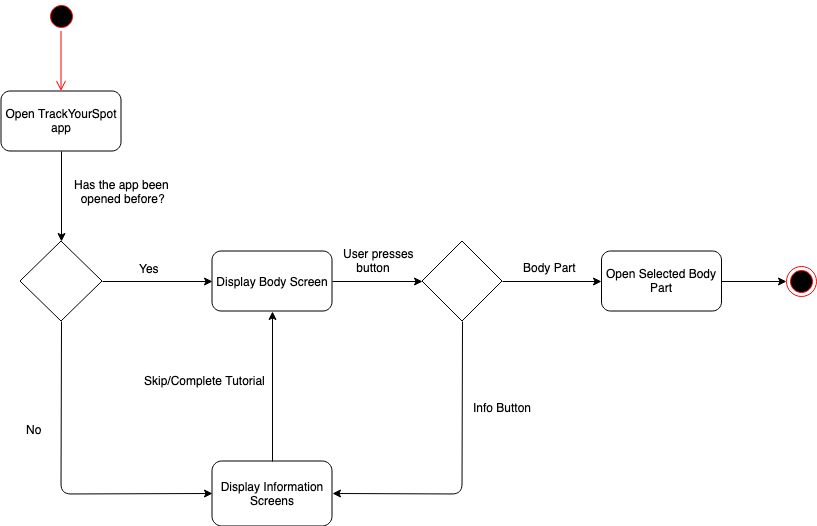
\includegraphics[width=1.2\textwidth, center]{figures/InfoDiagram.png}
    \caption{UML Activity Diagram for Info Screens}
    \label{fig:InfoDiagram}
\end{figure}

\subsection{CameraOpeningActivity} \label{sec:cameraarch}

\begin{figure}
    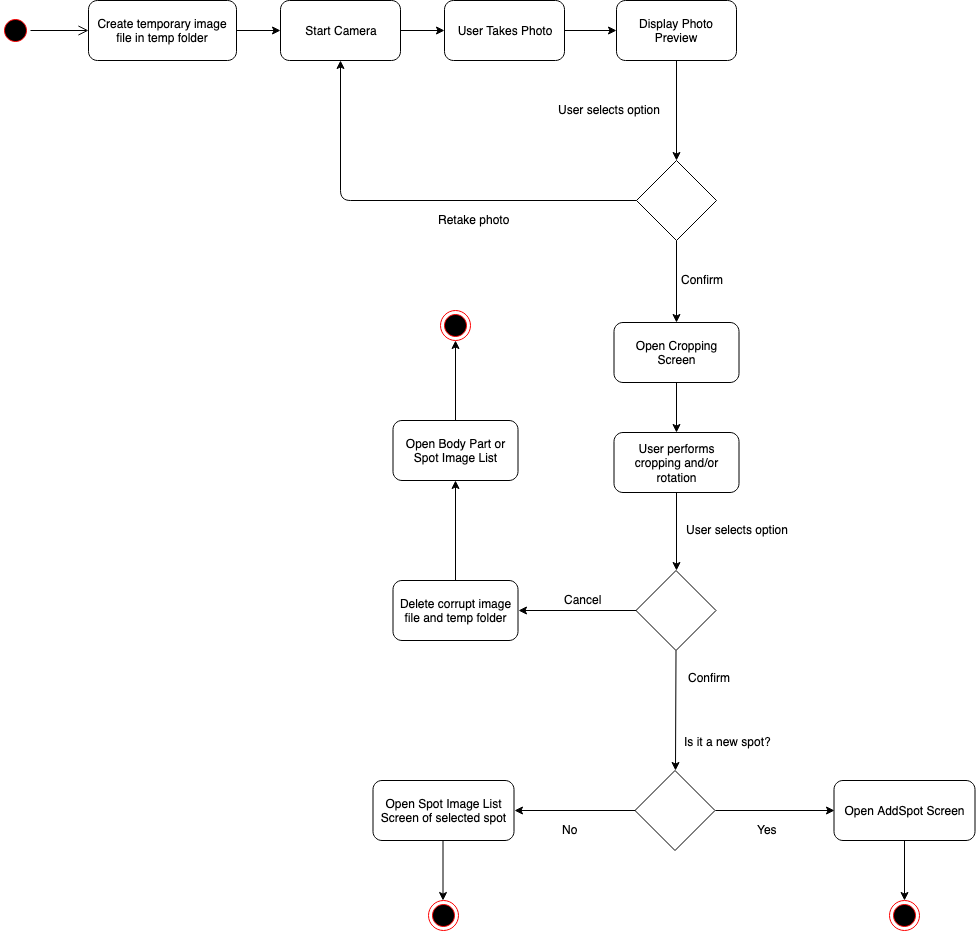
\includegraphics[width=1.2\textwidth, center]{figures/CameraScreen.png}
    \caption{UML Activity Diagram for the Camera Activity}
    \label{fig:CameraScreen}
\end{figure}
To explain the implementation of the \emph{OldSpotList} and \emph{SpotImageList} activities, we first have to break down the \emph{CameraOpeningActivity} class. This class was created so that the two mentioned activities could share the \code{createImageFile} and \code{dispatchTakePictureIntent} methods, avoiding any reduntant code. \code{createImageFile()} is used for creating a temporary empty image file in storage for the image to be taken, and \code{dispatchTakePictureIntent()} starts the actual camera app to save a new picture into this image file. The code has been adapted from the Android docs \cite{androiddevelopers3}, as these methods are widely used across any Photo taking app, comments have been added for clarification.

Take the \emph{OldSpotList} activity as an example. The user first selects a body part. They are then presented with the list of spots from that selected body part. Once the user presses the "+" button, the \code{ dispatchTakePictureIntent()} method would be called (Code Listing ~\ref{lst:dispatchTakePictureIntent}). The spotDirectory argument contains the path of where the photo will be saved, this could be something similar to:
\begin{verbatim}
/storage/emulated/0/Pictures/TrackYourSpot/front/torso/worryingspot/
\end{verbatim}
In line 8, the \code{createImageFile()} method first tries to create a temporary image file at the given path. It uses the current date and time to create a unique timestamp string (Code Listing ~\ref{lst:createImageFile}). This ensures no two images will have the same name. Next, the method checks if the spotDirectory path exists in storage, creating them through the \code{mkdirs()} method if needed. Once we have the directory, it creates the temporary file by concatenating the "JPEG\textunderscore" prefix, the timestamp, and the ".jpg" file extension. Back to the \code{dispatchTakePictureIntent} method, we need to find the \emph{URI} of the photoFile. The URI variable is passed on to the Intent in charge of starting up the Camera. For compatibility reasons, we have to check the device's Android version, as SDKs older than Lollipop require a different way of attaching intent data to the camera intent.

To see how this code interacts with the app's UI and navigation screens, take a look at Figure \ref{fig:CameraScreen}. The diagram also shows the paths the app takes if the user cancels the camera or cropping processes midway through. Since the camera process is based around temporary image files, these have to be dealt with accordingly.

\clearpage

\begin{lstlisting}[caption={Starting the Camera}, label={lst:dispatchTakePictureIntent}, language=Kotlin]
fun dispatchTakePictureIntent(spotDirectory: String) {
        Intent(MediaStore.ACTION_IMAGE_CAPTURE).also {
            takePictureIntent ->
            // Ensure that there's a camera activity to handle the intent
            takePictureIntent.resolveActivity(packageManager)?.also {
                // Create the File where the photo should go
                val photoFile: File? = try {
                    createImageFile(spotDirectory)
                } catch (ex: IOException) {
                    ... //Display error message
                }
                // Continue only if the File was successfully created
                photoFile?.also {
                    //Get the image file's URI
                    val photoURI: Uri = FileProvider.getUriForFile(
                            this, "my.package.name.provider", it)
                    //For compatibility issues, we need to check the device's
                    //Android version and add write permissions accordingly.
                    if (Build.VERSION.SDK_INT >= Build.VERSION_CODES.LOLLIPOP) {
                        takePictureIntent.addFlags(Intent.FLAG_GRANT_WRITE_URI_PERMISSION)
                    } else {
                        val clip = ClipData.newUri(contentResolver, "clipData", photoURI)
                        takePictureIntent.clipData = clip
                        takePictureIntent.addFlags(Intent.FLAG_GRANT_WRITE_URI_PERMISSION)
                    }
                    //Open Camera App
                    takePictureIntent.addFlags(Intent.FLAG_GRANT_READ_URI_PERMISSION)
                    takePictureIntent.putExtra(MediaStore.EXTRA_OUTPUT, photoURI)
                    startActivityForResult(takePictureIntent, OldSpotScreen.REQUEST_TAKE_PHOTO)
                }
            }
        }
    }
\end{lstlisting}



\begin{lstlisting}[caption={Creating an Image File}, label={lst:createImageFile}, language=Kotlin]
private fun createImageFile(spotDirectory: String): File {
        //Used for creating a unique name for the image file
        val timeStamp: String = SimpleDateFormat("dd-MM-yyyy_HHmmss").format(Date()) 
        //If needed, create the folder for the spot.
        val newDir = File(spotDirectory)
        if(!newDir.exists()) newDir.mkdirs()
        //Create a temporary image file
        return File.createTempFile(
                "JPEG_${timeStamp}_",
                ".jpg",
                newDir
        ).apply {
            //Saves the image path in String format for later use.
            currentFullPhotoPath = absolutePath
        }
\end{lstlisting}

\clearpage

%If you uncomment you have to explain it
%\begin{lstlisting}[caption={Camera and Cropping Output}, label={lst:cameraoutput}, language=Kotlin]
%//If Cropping has been done successfully
%if (resultCode == RESULT_OK && requestCode == UCrop.REQUEST_CROP) {
%    //Open Spot Image list screen for that specific spot
%    val intent = Intent(this, SpotImageList::class.java)
%    //Pass on spot name and directory to the image list
%   intent.putExtra("spotName", spotName)
%    intent.putExtra("spotDirectory", spotDirectory)
%    intent.putExtra("selectedBodyPart", selectedBodyPart)
%    intent.putExtra("selectedBodySide", selectedBodySide)
%    startActivity(intent)
%}
%
%//If Photo has been taken successfully
%f (requestCode == REQUEST_IMAGE_CAPTURE && resultCode == Activity.RESULT_OK) {
%    //Check if the photopath is valid (eg. is a jpg file in storage)
%    if (isValidPhotoPath(currentFullPhotoPath)) {
%        //Start uCrop cropping screen with specific UI properties
%        val cropOptions = UCrop.Options().apply {
%            setAllowedGestures(UCropActivity.NONE, UCropActivity.NONE, UCropActivity.NONE)
%            setShowCropGrid(false)
%            setToolbarColor(ContextCompat.getColor(applicationContext, R.color.blue))
%           setActiveWidgetColor(ContextCompat.getColor(applicationContext, R.color.blue))
%            setStatusBarColor(ContextCompat.getColor(applicationContext, R.color.blue))
%            setShowCropFrame(true)
%        }
%        //Choose the same source and destination for the cropped image (Overwrite it)
%       UCrop.of(Uri.parse("file://$currentFullPhotoPath"),
%                Uri.parse("file://$currentFullPhotoPath"))
%                .withAspectRatio(1.toFloat(),1.toFloat())
%                .withOptions(cropOptions)
%                .start(this)
%        }
%    }
%
%//If photo hasn't been taken (eg. user presses the back button)
%if (resultCode != RESULT_OK && isValidPhotoPath(currentFullPhotoPath)) {
%    //Delete the corrupt image file
%    File(currentFullPhotoPath).delete()
%    val intent = intent
%    finish()
%    startActivity(intent)
%}
%\end{lstlisting}

\subsection{Old Spot List Screen}

The old spot list screen extends the abstract class \emph{CameraOpeningActivity}. The code in this activity accomplishes the following tasks (See UML Diagram in Figure \ref{fig:OldSpotList}):
\begin{enumerate}
    \item Load all saved spots from storage
    \item Display spots with thumbnails and other info in a list format
    \item Start camera automatically or after the user's button click, checking permissions accordingly
\end{enumerate}
To display the list of spots of a selected body part, we run the algorithm in code listing \ref{lst:retrieveSpots}. This algorithm scans through directories and reads every spot name and path repeatedly. It first initialises empty arrays for spotNames, spotDetails, spotPaths and thumbnails (Lines 1-4). Using the  \code{walk()}  method, it loops through every file inside the \code{../TrackYourSpot/bodypart/} directory. Setting the \code{maxDepth} parameter to 1 ensures only the top level folders inside these are read, in other words, only the spot names, but nothing inside these directories. Index 0 contains the root folder, therefore we choose to ignore it as it does not provide a spotName. Inside each of these spotName folders, we perform a 1-depth walk again, this time selecting only the file at index 1, which would contain the first image taken of a spot. We then use this image's path to display a thumbnail for each spot.

\clearpage
\begin{lstlisting}[caption={Loading Old Spots}, label={lst:retrieveSpots}, language=Kotlin]
var spotNames = emptyArray<String>() //Spot Names
var spotDirectories = emptyArray<String>() //Spot paths without jpg file
var spotThumbnails = emptyArray<Bitmap>() //Spot thumbnail paths
var numberOfSpots = 0 //Counter for later use
File(spotListDirectory).walk().maxDepth(1).forEachIndexed { index, file ->
    if (index != 0) { //Ignore the root folder
        numberOfSpots++
        val spotName = file.toString().removePrefix(spotListDirectory)
        spotNames += spotName //Add spot to list of spot names
        spotDirectories += "$spotListDirectory$spotName/" //Add directory
        val filesInFolder = File("$spotListDirectory/$spotName/").walk().maxDepth(1).toList()
        //Grab first image of each spot folder
        spotThumbnails += if (filesInFolder.size>1) {
            BitmapFactory.decodeFile(filesInFolder[1].absolutePath)
        } else { //Show question mark icon if image is missing.
            BitmapFactory.decodeResource(this.resources, R.drawable.questionmark)
        }
    }
}
\end{lstlisting}

\begin{figure}
    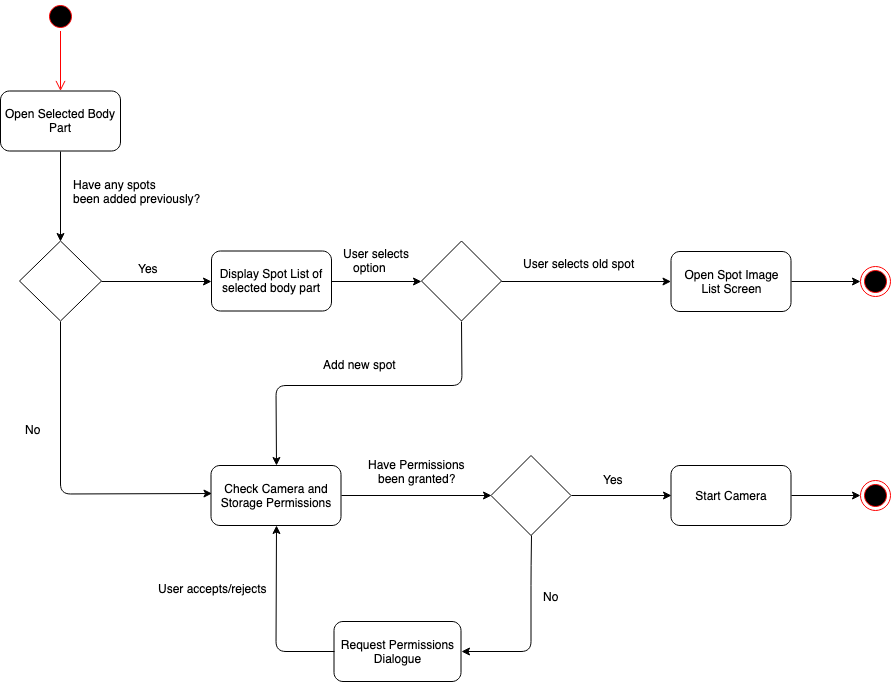
\includegraphics[width=1.2\textwidth, center]{figures/OldSpotList.png}
    \caption{UML Activity Diagram for the Old Spot's screen}
    \label{fig:OldSpotList}
\end{figure}

\subsection{Spot Image List}

This activity also extends the CameraOpeningActivity class, similarly to the \emph{OldSpotScreen}. This screen also makes use of the camera when a user elects to add a new photo of an existing spot. Figure \ref{fig:SpotImageList} depicts the process of the opening the screen, with the different paths available to the user. When the user opens the Spot Image List of a particular spot, all the photos of a spot are read from storage. This algorithm is displayed in Code Listing \ref{lst:loadingspotimages}. In a similar way to the algorithm in Code Listing \ref{lst:retrieveSpots}, spots are first loaded from storage with the \code{walk()} method. This creates a list of \code{imageFiles}, each of which we decode into an image path and thumbnail. We also initialise an array \code{selectedSpotBooleanList} to keep track of which images are being selected by the user (to compare).

Following the UML Diagram, the user can press the "+" button to add a new photo. If the goal is to compare two images, the user can either:
\begin{itemize}
    \item Press on an image for more than 2 seconds
    \item Click the "Compare" button on the toolbar
\end{itemize}
Both of these options would launch the \emph{Contextual Action Bar}, this is a toolbar that substitutes the default toolbar when a specific action takes place. It allows the user to select images from the list. If exactly two images are selected, a "Compare" button lights up, indicating the user can compare the images.

\begin{figure}
    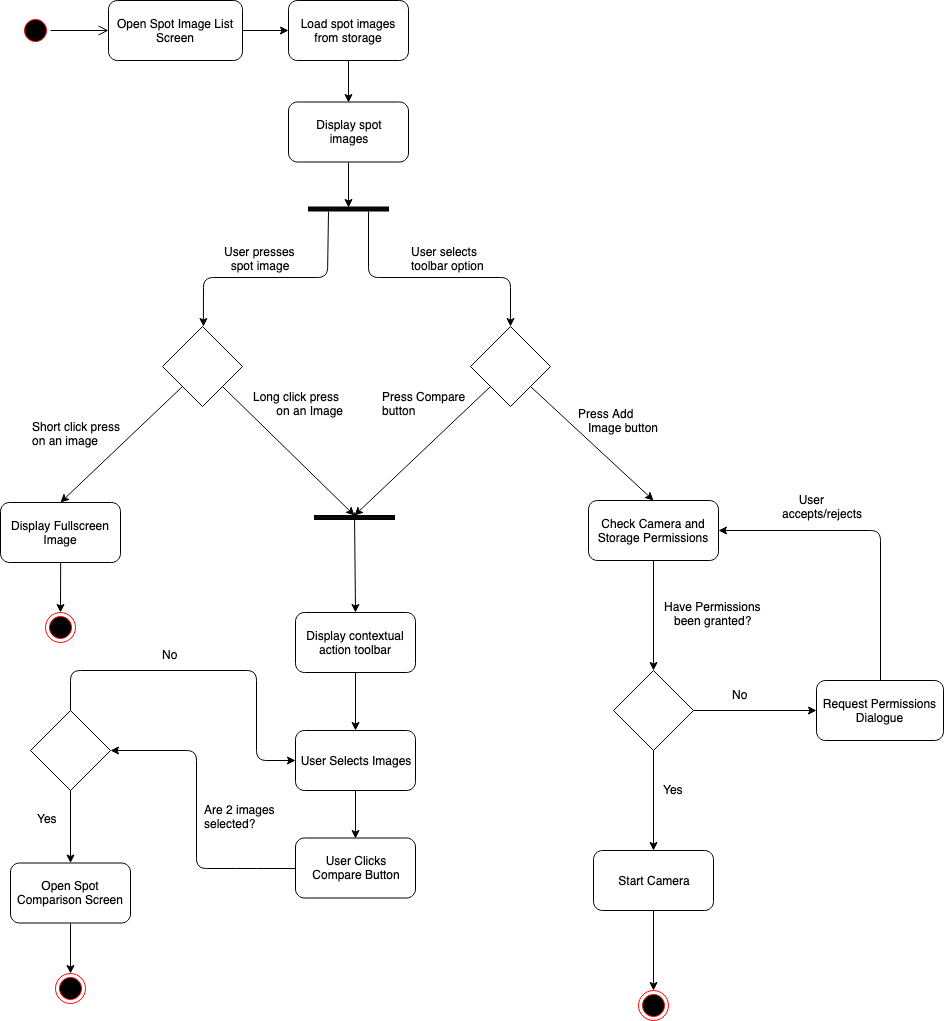
\includegraphics[width=1.2\textwidth, center]{figures/SpotImageList.png}
    \caption{UML Activity Diagram for the Spot Image List}
    \label{fig:SpotImageList}
\end{figure}
\begin{lstlisting}[caption={Loading spot images to compare}, label={lst:loadingspotimages}, language=Kotlin]
//Initialise arrays for each photo's path and thumbnails
var fullImagePaths = emptyArray<String>()
var imageThumbnails = emptyArray<Bitmap>()
//Loop through images in the selected spot's directory
val imageFiles =  File(spotDirectory).walk().maxDepth(1).toList()
for (i in 2..imageFiles.size) {
    fullImagePaths += imageFiles[i-1].toString()
    imageThumbnails += BitmapFactory.decodeFile(imageFiles[i-1].absolutePath)
}
numberOfImages = fullImagePaths.size
//Initialise dynamic array to keep track of which images are selected
val selectedSpotBooleanList = arrayOfNulls<Boolean>(fullImagePaths.size)
//By default, no images are selected 
Arrays.fill(selectedSpotBooleanList, java.lang.Boolean.FALSE)
\end{lstlisting}

\subsection{AddSpot Screen}

When the user chooses to add a new spot to a body part, they first take a photo, crop it to the desired dimensions, and is then redirected to this screen, the \emph{AddSpot} Activity. As shown in figure \ref{fig:AddSpot}, they are asked to input a name for this spot, displaying appropriate error messages if the name violates any of the following properties:
\begin{itemize}
    \item Spot name is not left blank
    \item Spot name is under 20 characters
    \item Spot name contains only letters and numbers
\end{itemize}
This ensures stability when spot folders are created in storage, as any unrecognised characters (e.g. @, !, \$) could easily cause errors. The rules were devised following advice on folder naming conventions from \cite{santaguida_2011}. If the name satisfies these conditions, the spot folder is created in storage, substituting spaces for dashes ("-") to further comply with good practices.

The algorithm in charge of this task is shown in Code Listing \ref{lst:addSpot}. Running through the algorithm; a \code{photoDirectory} string is created, populating it by replacing the "temp" text with the body side, body part, and given spot name. This is the first step to move the image file from the temporary folder into a new folder named after the new spot. Next, a directory \code{newDir} is created at this path (making sure it doesn't exist yet through the \code{exists()} command). Once the folder is created, we proceed to move the image by modifying its path with the \code{renameTo} method. We then delete the (now empty) \code{tempfolder}, as the file has been succesfully moved.

\begin{figure}
    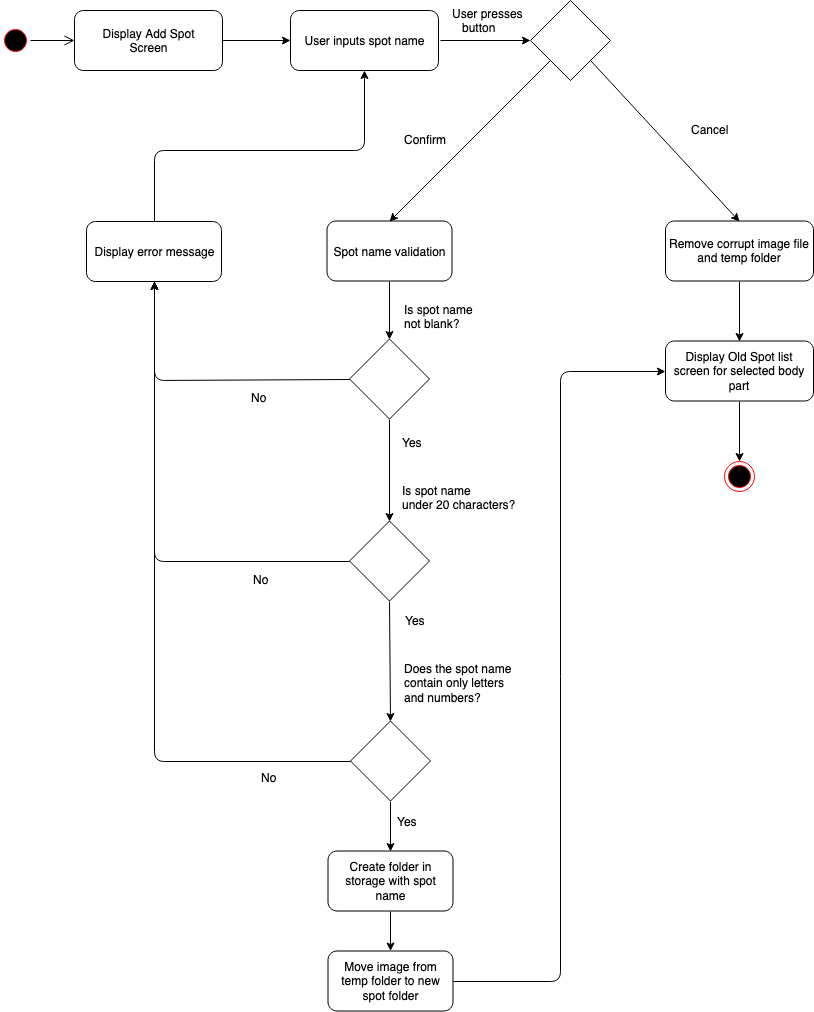
\includegraphics[width=1.2\textwidth, center]{figures/AddSpot.png}
    \caption{UML Activity Diagram for the AddSpot Activity}
    \label{fig:AddSpot}
\end{figure}

\begin{lstlisting}[caption={Adding a Spot}, label={lst:addSpot}, language=Kotlin]
private fun moveImageFile(spotImageName: String, 
newSpotName: String, selectedBodySide: String, selectedBodyPart: String) {
    val photoDirectory = fullPhotoPath.removeSuffix(spotImageName)
    //Move image from temp folder to a new *newSpotName* folder
    val newDirPath = 
    photoDirectory.replace("temp", "$selectedBodySide/$selectedBodyPart/$newSpotName")
    val newDir = File(newDirPath)
    //Check if the directory exists already, create it otherwise
    if(!newDir.exists()) newDir.mkdirs()
    //Make app available in the device's Gallery
    Intent(Intent.ACTION_MEDIA_SCANNER_SCAN_FILE).also { mediaScanIntent ->
        val f = File(fullPhotoPath)
        mediaScanIntent.data = Uri.fromFile(f)
        sendBroadcast(mediaScanIntent)
        //Rename the file to the new path
        f.renameTo(File(newDirPath + spotImageName))
        //Delete the temporary folder
        val tempFolder = File(photoDirectory)
        deleteRecursive(tempFolder)
    }
}
\end{lstlisting}

\subsection{Compare Screen}
The workflow of the Compare Screen is very straightforward. Following the UML diagram in Figure \ref{fig:CompareScreen}, once the two images are displayed, the user's only options are to go back to the image list or email the two photos. If the user wanted to email the photos, they would press the email button, at which point the default email app is initiated, automatically creating a new message with the two attachments. Once the user sends the email, the compare screen opens again, displaying a \emph{Toast} message (short pop-up message that fades away after 2 seconds).

\begin{figure}
    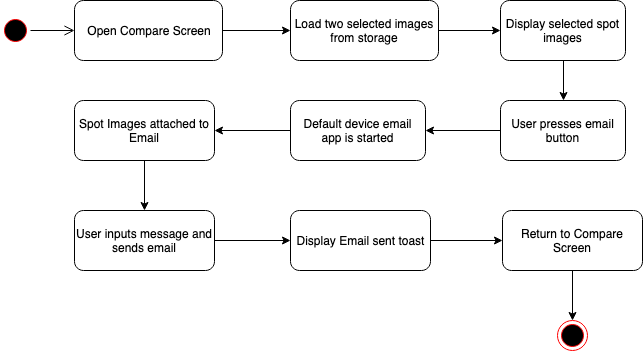
\includegraphics[width=1.2\textwidth, center]{figures/CompareScreen.png}
    \caption{UML Activity Diagram for the CompareScreen Activity}
    \label{fig:CompareScreen}
\end{figure}

%If you outcomment then gotta explain
%\begin{lstlisting}[caption={Starting the comparison}, label={lst:startingcomparison}, language=Kotlin]
%//Initialise contextual action toolbar to allow user to select images
%mActionModeCallback = object : AbsListView.MultiChoiceModeListener { 
%    //This method is called whenever an item is selected or deselected
%    override fun onItemCheckedStateChanged(mode: ActionMode, 
%    position: Int, id: Long, checked: Boolean) {
%       //Update list of selected spots array
%        selectedSpotBooleanList[position] = checked
%        val checkedItemCount = listView.checkedItemCount
%        //Allow pressing the compare button if exactly 2 images are selected
%        mode.menu.findItem(R.id.compare).isEnabled = checkedItemCount == 2
%    }
%    //This method is called when the user presses a button in the
%    //contextual action toolbar.
%    override fun onActionItemClicked(mode: ActionMode, item: MenuItem): Boolean{
%        return when (item.itemId) {
%            //When the user presses the "compare" button
%            R.id.compare -> {
%                //Initialise array of indices of the images to compare
%                var spotIndicesToCompare = emptyArray<Int>()
%                //Loop through array of selected spots
%                (0 until selectedSpotBooleanList.size)
%                        //If a spot is selected, save it's index
%                        .filter { selectedSpotBooleanList[it]==true }
%                        .forEach { spotIndicesToCompare+= it }
%                //Get image paths for both spots to be compared
%                val firstSpotToCompare = fullImagePaths[spotIndicesToCompare[0]]
%                val secondSpotToCompare = fullImagePaths[spotIndicesToCompare[1]]
%                //Open the comparison screen and send info of selected sports
%                val intent = Intent(this@SpotImageList, CompareSpotScreen::class.java)
%                intent.putExtra("firstSpotToCompare", firstSpotToCompare)
%                intent.putExtra("secondSpotToCompare", secondSpotToCompare)
%                intent.putExtra("spotName", spotName)
%                intent.putExtra("spotDirectory", spotDirectory)
%                intent.putExtra("selectedBodyPart", selectedBodyPart)
%                intent.putExtra("selectedBodySide", selectedBodySide)
%                startActivity(intent)
%                //Return true if the click event has been handled
%                true
%            }
%            else -> false
%        }
%    }
%\end{lstlisting}

\section{Data Flow}
Most mobile applications require constantly sending information from one screen to another. This is done through the use of \emph{Intents}. In plain terms, an Intent is an intention to perform an action, or in other words, "a messaging object you can use to request an action from another app component" \cite{intents}. Intents can have data extras, these are key-value pairs such as strings or booleans. In the \emph{TrackYourSpot} context, the main data being attached to intents is:
\begin{itemize}
    \item \textbf{selectedBodySide} - "front" or "back"
    \item \textbf{selectedBodyPart} - "head", "back", "torso", "leftarm", "rightarm", "leftleg", "rightleg"
    \item \textbf{spotName} - User defined spot name such as "Spot1"
    \item \textbf{spotDirectory} - Directory of a spot in storage such as "/storage/emulated/0/Pictures/TrackYourSpot/front/torso/Spot1/"
    \item \textbf{spotListDirectory} - Directory of a body part in storage such as "/storage/emulated/0/Pictures/TrackYourSpot/back/head/"
    \item \textbf{spotImageName} - File name of a particular image such as "JPEG\_20190113\_133157.jpg"
    \item \textbf{fullPhotoPath} - Full path of an image such as "/storage/emulated/0/Pictures/TrackYourSpot/front/torso/Spot1/JPEG\_20190113\_133157.jpg"
\end{itemize}
An example intent can be found in Code Listing \ref{lst:intentdataflow}. In that particular example, the intent takes the user from the OldSpotList to the Addspot screen. Note how variables and intent data labels are equal. This has been done to ensure consistency across screens and make sure it is clear what every variable represents in different screens.

\begin{lstlisting}[caption={Intent Dataflow for the AddSpot class}, 
label={lst:intentdataflow}, language=Kotlin]
val intent = Intent(this, AddSpot::class.java)
intent.putExtra("selectedBodySide", selectedBodySide)
intent.putExtra("selectedBodyPart", selectedBodyPart)
intent.putExtra("spotListDirectory", spotListDirectory)
intent.putExtra("spotImageName", spotImageName)
intent.putExtra("fullPhotoPath", currentFullPhotoPath)
startActivity(intent)
\end{lstlisting}
\section{File Structure} \label{sec:filestructure}
The file structure for the app is relatively simple. Initially, images are stored in the default picture directory defined by each device. To identify this path, a File object needs to be created by calling the following method: \begin{verbatim}
getExternalStoragePublicDirectory(Environment.DIRECTORY_PICTURES)
\end{verbatim}
This file's path can then be identified by calling the inbuilt \code{getAbsolutePath()} method from the File.java class. 

\par Once we're located inside the absolute directory, pictures in .jpg format are saved in a \code{../bodySide/bodyPart/spotName}
folder hierarchy, where bodySide can be one of "front" or "back", bodyPart refers to the selected body part of a spot, it can take any of the following labels:
\begin{itemize}
    \item \textbf{Front} - Head, Torso, Rightarm, Leftarm, Rightleg, Leftleg
    \item \textbf{Back} - Head, Back, Rightarm, Leftarm, Rightleg, Leftleg
\end{itemize}
The spotName is the user defined name given to the spot at the time of adding the first image. Spot folders are created on demand, so the \code{../front/leftarm/worryingspot} folder will only be generated when the user takes a picture of a spot and gives it a name. Therefore, a typical folder structure could look like Figure~\ref{fig:filestructure.png}.
\begin{figure}
    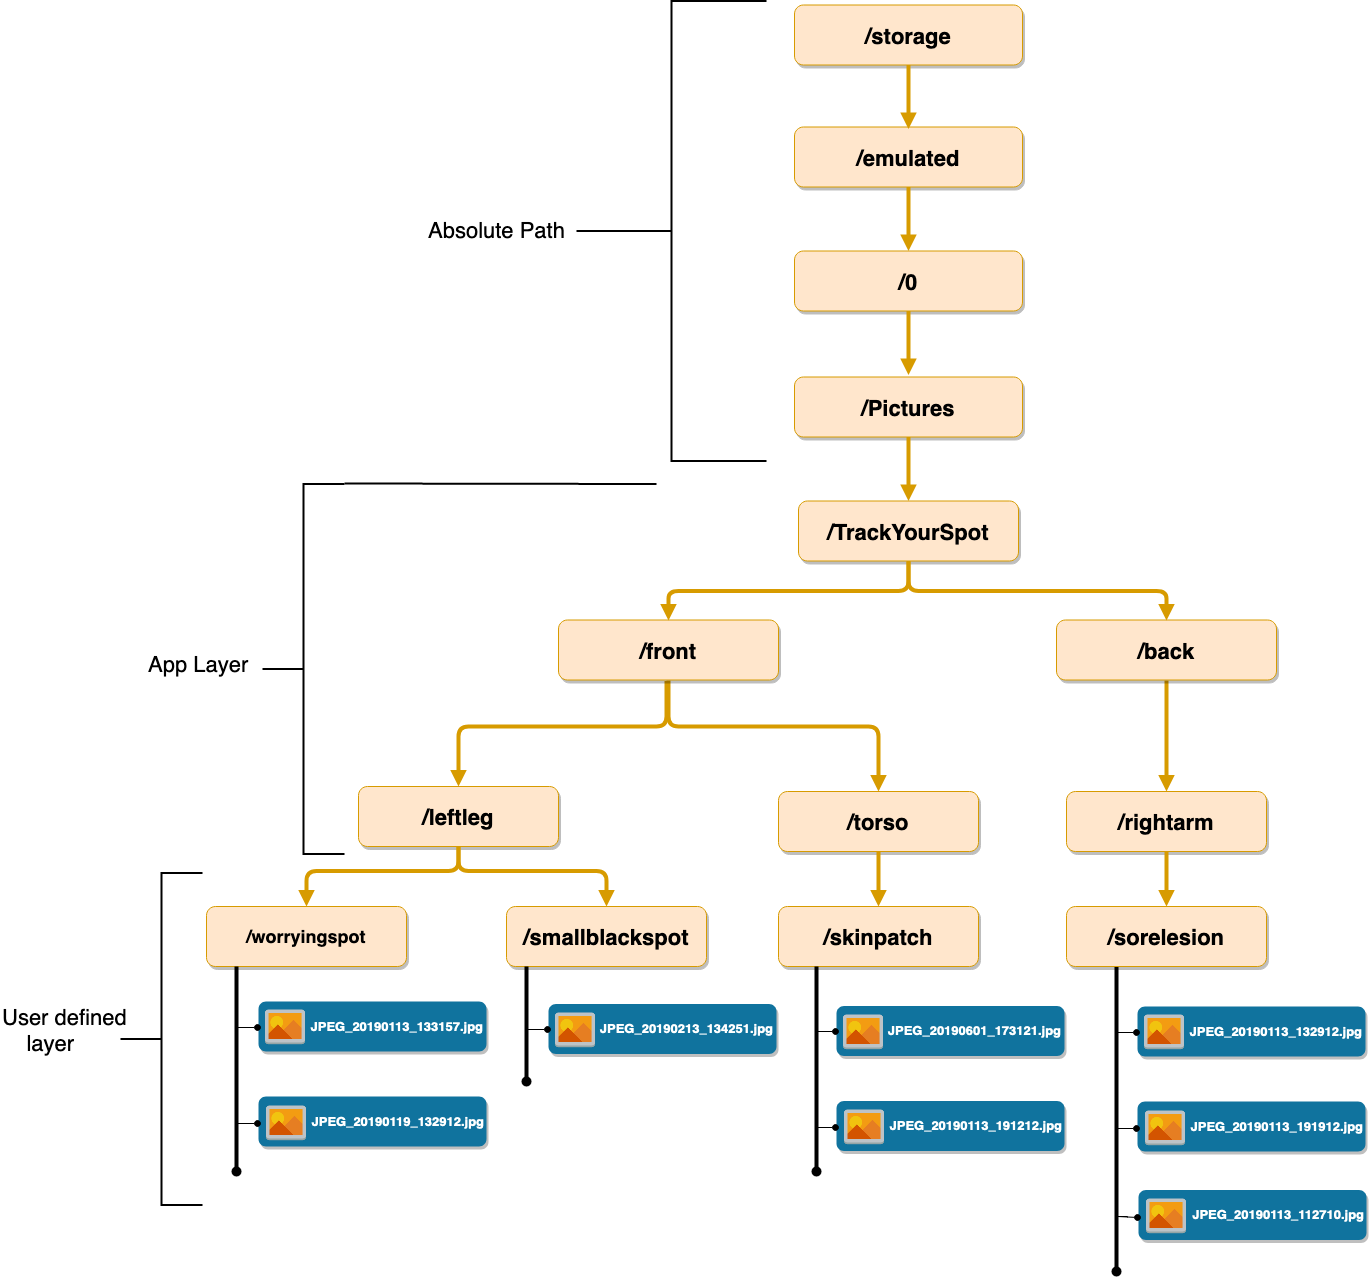
\includegraphics[width=1.2\textwidth, center]{figures/filestructure.png}
    \caption{A typical folder hierarchy showing folder layers within the user's device}
    \label{fig:filestructure.png}
\end{figure}
\par Another component of this file hierarchy are \code{/temp} folders. These temporary folders are only generated when pictures are not saved correctly due to the user closing the app without naming the spot, causing the spot to not be saved to the correct location.